\section{Methodology}

\subsection{Server Environment}
The implementation was carried out on a remote SSH server running Ubuntu.
Both srsRAN Project and Open5GS were installed and configured on this server.

\subsection{Open5GS Setup}
Open5GS was installed following the official documentation. The core network 
components including AMF, SMF, UPF, and other network functions were configured 
to support 5G SA (Standalone) operation.

\subsection{srsRAN Project Setup}
The srsRAN Project gNB (next generation NodeB) was configured to connect to 
the Open5GS core. Configuration files were modified to set the correct PLMN, 
AMF address, and radio parameters.

\subsection{Network Architecture}
Figure \ref{fig:architecture} shows the 5G network architecture implemented
using srsRAN Project and Open5GS.

\begin{figure}[h!]
    \centering
    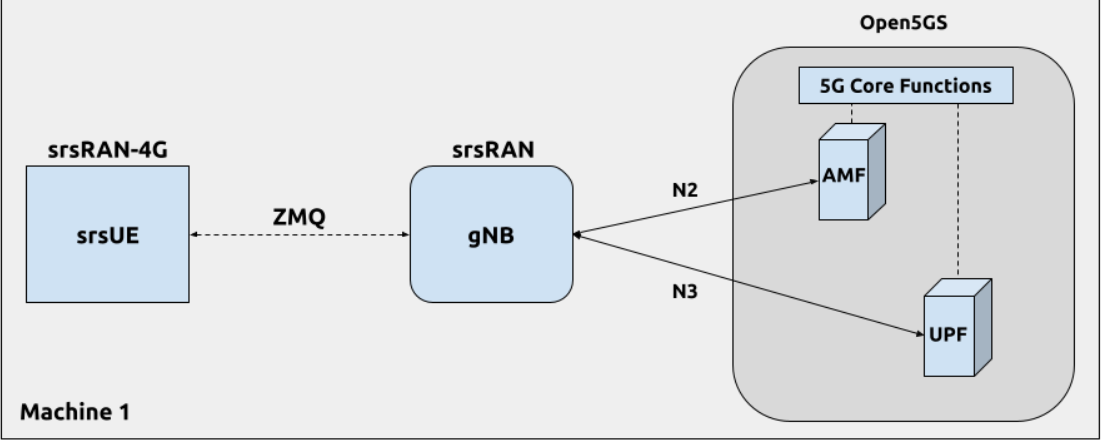
\includegraphics[width=0.9\textwidth]{figures/architecture.png}
    \caption{5G Network Architecture with srsRAN and Open5GS}
    \label{fig:architecture}
\end{figure}
```